\documentclass[conference]{IEEEtran}
\usepackage{cite}
\usepackage{amsmath,amssymb,amsfonts}
\usepackage{graphicx}
\usepackage{textcomp}
\usepackage[colorlinks=true,linkcolor=blue,citecolor=blue,urlcolor=blue]{hyperref}
\usepackage{url}
\usepackage{float}

\begin{document}

\title{Efficient Point Prompt Optimization for Segmentation using Reinforcement Learning}

\author{
\IEEEauthorblockN{Xeerak Muhammad, Jacob Vaught, Jacob Whisenant}
\IEEEauthorblockA{CSCE 775 --- February 25, 2026}
}

\maketitle

\section{Introduction}

The Segment Anything Model (SAM)~\cite{Kirillov2023SAM} demonstrated that a single foundation model can segment arbitrary objects when guided by user-provided prompts such as points, boxes, or masks. Among these, point prompts are the most lightweight, requiring only a click on the target object, yet their placement significantly affects segmentation quality. A point near the center of a salient region typically produces a tight mask, while a poorly placed point can yield partial or incorrect segmentation. Manually selecting effective point prompts for every image is impractical at scale, motivating automated approaches.

Fully supervised segmentation methods address this by training on large pixel-level annotated datasets, but acquiring such annotations is expensive and labor-intensive. Few-shot methods reduce the annotation burden by leveraging a small support set to segment novel classes, yet they still depend on carefully chosen exemplars and often degrade on out-of-distribution data. Recent work has framed point prompt selection as a reinforcement learning (RL) problem, where an agent learns to choose prompts that maximize segmentation quality without requiring dense annotations for every target image. We build on this line of work by addressing limitations in the state representation, reward signal, and candidate generation stages of an existing RL-based prompt optimization pipeline.

\section{Approach}

Figure~\ref{fig:pipeline} illustrates our proposed pipeline. We plan to extend the Plug-and-Play Prompt Optimization (PPO) pipeline by Liu et al.~\cite{Liu2025PPO}, which optimizes point prompt selection for SAM-based one-shot segmentation. Their pipeline constructs a dual-space heterogeneous graph where nodes represent candidate prompt locations and five edge types encode pairwise distances in both DINOv2 feature space and pixel coordinate space. The agent selects a subset of prompts by restoring or removing nodes, receiving rewards based on changes in mean edge weights that encourage semantic cohesion, foreground-background separation, and spatial spread. The optimized prompt subset is then passed to SAM for segmentation. Although the paper describes a Q-network as the policy network, the released implementation uses a tabular Q-table. We identify three limitations in this implementation and propose corresponding improvements.

\begin{figure*}[t]
\centering
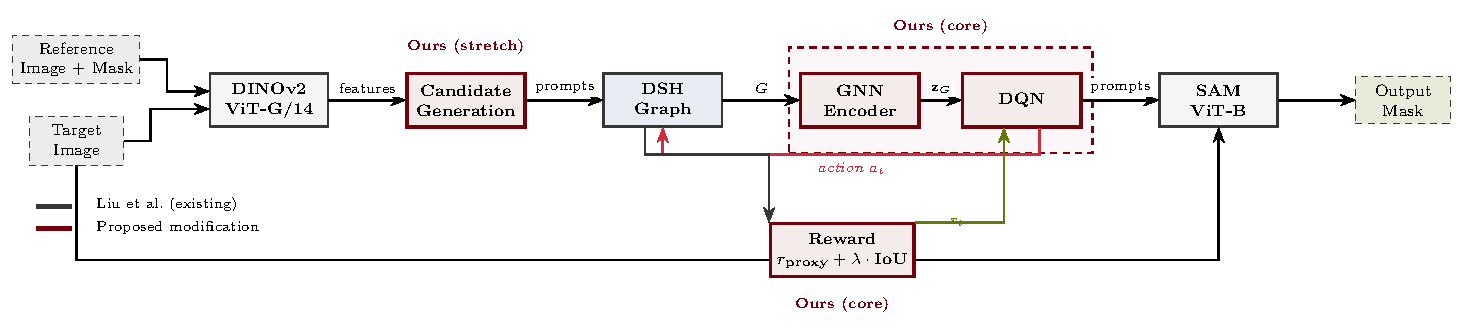
\includegraphics[width=\textwidth]{figures/fig_proposal_pipeline.pdf}
\caption{Proposed pipeline. Garnet-bordered components indicate our modifications to the Liu et al.~\cite{Liu2025PPO} baseline. The GNN encoder and DQN replace the original tabular Q-table, the reward function adds an IoU term, and the candidate generation stage is a stretch goal.}
\label{fig:pipeline}
\end{figure*}

First, the tabular Q-table cannot generalize across similar graph configurations. The Q-table state keys are tied to specific graph object instances, so when the graph resets each episode, all prior Q-values become orphaned. Only the replay buffer persists across episodes, but replaying those transitions updates Q-values for states that no longer exist. Furthermore, the state representation compresses the entire graph into five scalar statistics (mean edge weights per type), discarding all topological information. We will replace the Q-table with a \textbf{Graph Neural Network (GNN)} encoder that operates directly on the graph structure, producing a graph-level embedding that feeds into a \textbf{Deep Q-Network (DQN)}. This enables generalization across episodes through learned function approximation while preserving structural information about prompt arrangements and their relationships.

Second, the reward function optimizes a geometric proxy without any direct measure of segmentation quality. In our reproduction experiments, the highest segmentation IoU did not correspond to the highest cumulative reward, indicating that the proxy can diverge from the true objective. We will incorporate an \textbf{Intersection over Union (IoU)} term directly into the reward function by periodically evaluating the current prompt set against a small set of ground-truth masks during training, requiring substantially less annotation than fully supervised methods.

Third, if time permits, we plan to investigate improvements to the candidate prompt generation step. The current pipeline generates initial prompts via coarse segmentation sampling or feature matching, neither of which incorporates learned discriminative information about what makes a good prompt location for a given target class. We will explore lightweight learned sampling strategies that leverage DINOv2 features to produce higher-quality initial candidate sets before RL optimization begins.

\section{Evaluation}

We will evaluate segmentation quality using the mean Dice Similarity Coefficient (mDSC) and mean Hausdorff Distance (mHD). Our baselines fall into two categories: RL-based prompt optimization methods (Liu et al.~\cite{Liu2025PPO}, AlignSAM~\cite{Huang2024AlignSAM}) and prompt-based few-shot segmentation methods (Matcher~\cite{Liu2023Matcher}, VRP-SAM~\cite{Sun2024VRPSAM}, PerSAM~\cite{Zhang2023PerSAM}, SAM2-UNet~\cite{Xiong2024SAM2UNet}). All methods will be compared under the same one-shot setting and datasets. We will also conduct a learning curve analysis by varying the number of ground-truth masks available to the RL agent's IoU reward during training (1, 3, 5, 10 masks per class) to measure how segmentation performance scales with minimal supervision. Finally, we will perform an ablation study evaluating three configurations: GNN-DQN with the original proxy reward, GNN-DQN with the IoU reward term, and, if time permits, the full pipeline with improved candidate generation, to isolate the contribution of each proposed modification.

We plan to benchmark on two natural and two medical image datasets. The natural image datasets are FSS-1000~\cite{Li2020FSS1000} (10,000 images, 1,000 classes) and VOC2012~\cite{Shetty2016PascalVOC} (4,396 images, 20 object classes). The medical image datasets are ISIC2018~\cite{Codella2019ISIC} (2,594 dermatoscopic images for lesion segmentation) and Kvasir~\cite{Jha2020KvasirSEG} (1,000 images for colorectal polyp segmentation).

\section{Conclusion}

We propose three improvements to the Plug-and-Play PPO pipeline for RL-based point prompt optimization. A GNN encoder paired with a DQN replaces the tabular Q-table and its lossy five-scalar state representation, preserving graph structure across episodes. An IoU reward term supplements the geometric proxy to align training directly with segmentation quality. If time permits, we will also investigate learned candidate generation to improve the initial prompt set. We plan to evaluate these contributions through an ablation study, a learning curve analysis over varying annotation budgets, and comparisons against both RL-based and few-shot segmentation baselines on natural and medical image datasets.

\bibliographystyle{IEEEtran}
\bibliography{references}

\end{document}
